%! Author = smf
%! Date = 4/30/23

% Preamble
\documentclass[11pt]{article}

% Packages
\usepackage{amsmath}
\usepackage{graphicx}

\author{Mingfei Shi}
\title{Transformer Part}
\date{\today}


% Document
\begin{document}
    \maketitle
    \newpage
\section{What are the Transformer and attention mechanisms}\label{sec:what-are-the-transformer-and-attention-mechanisms}

\paragraph{Self-attention} Relate different positions of a single sequence to compute a representation of the same sequence.
    Each element becomes query, key, and value from the input embeddings by multiplying by a weight matrix.

    The goal is to learn how to pick relevant information from input data.
    Then they create three vectors from each of the encoder's input values(query, key, value), and calculate a score for how much
    to focus on each part of the input when we encode words at specific positions.
    The idea is to select a value (referenced by a key) relevant to a query.

    \[Attention(Q, K, V) = softmax\left(\frac{QK^T}{\sqrt {d_k}}V\right),\]
    \subparagraph{Multi-Head Attention} Inputs consist of queries , keys of dimension $d_k$ and values of dimension $d$.
    Stack linear layers (weight matrices without biases) that are independent each for keys, queries and values.
    Concatenate output of attention heads to form (plus non-linearity) output layer.
    Then they get Multi-Head Attention.
    \[MultiHead(Q, K, V) = Concat(head_1, \cdots, head_h)W^O,\]
    where $head_i = Attention(QW_i^Q, KW_i^K, VW_i^V).$
    Focus on different positions, and no longer need to oversaturate one attention mechanism.

    \subparagraph{Positional Encoding} We need for information about the position and order of tokens in a sequence.
    Vectors of representing position of each token should be fixed of learned.
    Element wise addition the position embedding to the word embedding vector.
    In paper, they use
    \begin{gather*}
        PE_{(pos, 2i)} = \sin\left(\frac{pos}{10000^{2i/d_{model}}}\right),\\
        PE_{(pos, 2i+1)} = \cos\left(\frac{pos}{10000^{2i/d_{model}}}\right),\\
    \end{gather*}
    where $pos$ is the position and $i$ is the dimension.
    
    \begin{figure}[htbp]
        \centering\label{fig:figure}
        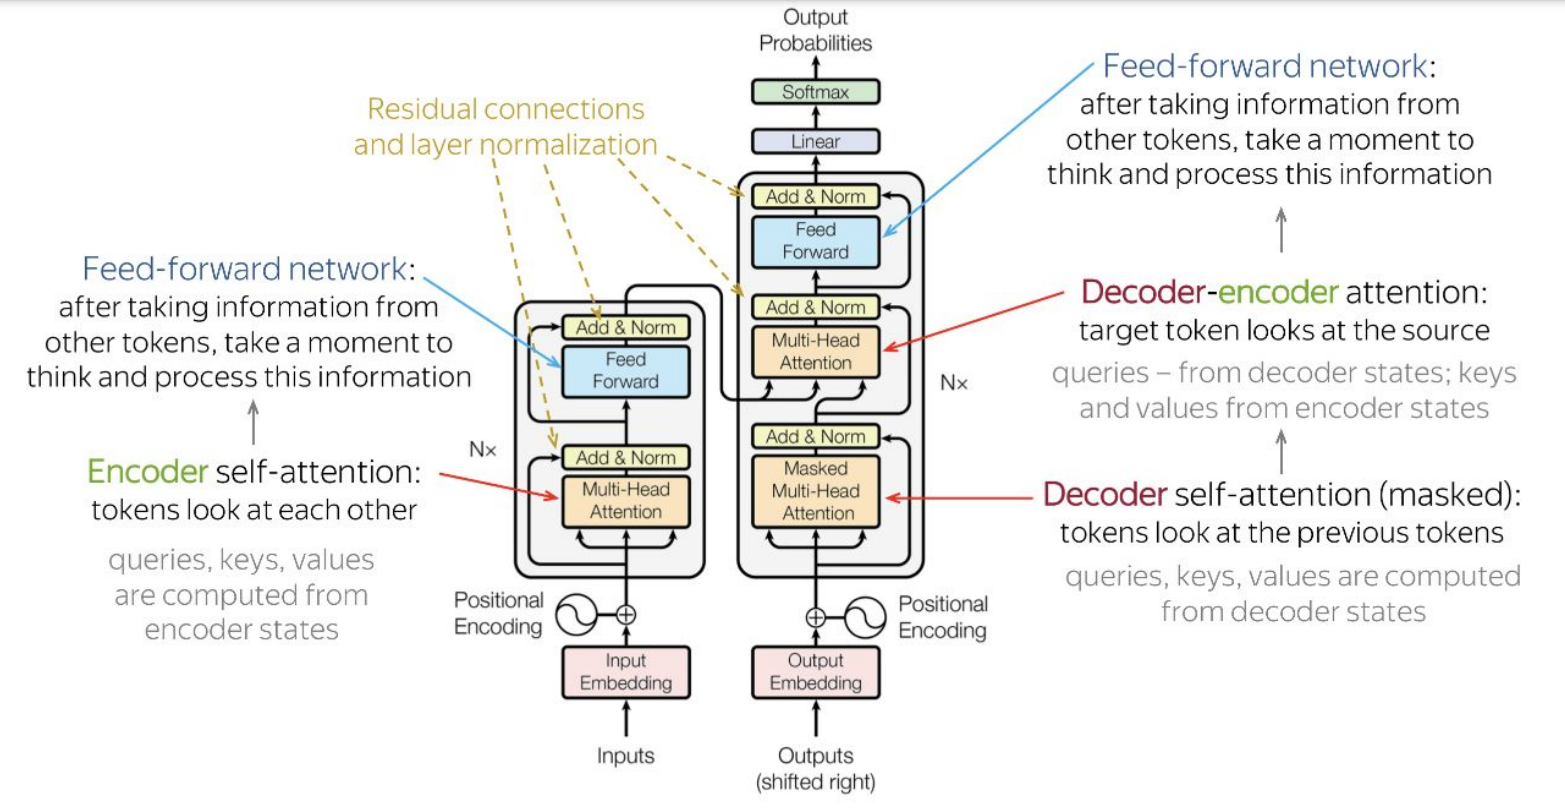
\includegraphics[scale=0.4]{figs/fig1}
        \caption{Full architecture}
    \end{figure}




\end{document}